%%%
% set up document type
%%%
\documentclass[12pt]{article}

%%%
% declare all packages
%%%
\usepackage[left=25mm, top=20mm, right=25mm, bottom=30mm,nohead,nofoot]{geometry} 

\usepackage[T2A]{fontenc}
\usepackage[utf8]{inputenc}
\usepackage[english, russian]{babel}

\usepackage{graphics, graphicx}

\usepackage{url}
\usepackage{hyperref}

\usepackage{amssymb,latexsym} 
\usepackage{MnSymbol}
\usepackage{mathrsfs}

\usepackage[nottoc,numbib]{tocbibind}
\usepackage{float}
\usepackage{listings}
\usepackage{multirow}
\usepackage{hhline}
\usepackage{delarray}

\usepackage{color,colortbl}

% \usepackage{verbatim}
%%%
% document settings
%%%
\setcounter{tocdepth}{4}
\graphicspath{ {./pic/} }

\renewcommand{\listoffigures}{\begingroup  % add number to list of graphics
\tocsection
\tocfile{\listfigurename}{lof}
\endgroup}
\renewcommand{\listoftables}{\begingroup  % add number to list of tables
\tocsection
\tocfile{\listtablename}{lot}
\endgroup}

%******************************************************************
%******************************************************************
\begin{document}

\begin{titlepage}
	\center
		Санкт-Петербургский Политехнический 
		университет \\ Петра Великого\\
		Институт прикладной математики и механики
		\\ \textbf{Высшая школа прикладной математики и вычислительной физики}

	\vfill ~
	\textbf{
		\\ \large ЛАБОРАТОРНАЯ РАБОТА №3
	}
	\\	на тему 
	\\ "Метод конечных объёмов для уравнений эллиптического типа"
	\\ по дисциплине
	\\ "Конечно-разностные и сеточные методы"

	\vfill ~

	Выполнил студент гр. \textbf{3630102/60101} \\
	\textbf{Лансков.Н.В.} \\ 

\vfill

{\large}	Санкт-Петербург
\\ 2020
\end{titlepage}

%%%
% Table of conetnts 
%%%

\tableofcontents 
\newpage
\listoffigures
\newpage
\listoftables
\newpage

%%%
% Text
%%%
\section{Постановка задачи}

Будем решать задачу:

$$
\begin{cases}
-\dfrac{\partial}{\partial x}\left( a(x,y) \dfrac{\partial u}{\partial x}\right) - \dfrac{\partial}{\partial y}\left( b(x,y) \dfrac{\partial u}{\partial y}\right) + q(x,y)u = f(x,y)
\\ \\
0 < \alpha < a, b < \beta; 0 < q_m < q; & (x,y) \in [3, 3.4] \times [1, 1.4] = \Omega
\\ \\
u|_{\partial \Omega} = g(x, y)
\end{cases}
$$

В данной лабораторной исследуется задача со следующими параметрами:
$$
\begin{cases}
a(x,y) = x + y \\ 
b(x,y) = 1 + xy \\
q(x,y) = x^4 \\
g(x,y) = cos(2x) \cdot e^{-3y} \\
f(x,y) = 3xcos(2x)e^{-3y}+4xsin(2x)e^{-3y} - 9cos(2x)e^{-3y}(xy + 1) + x^4cos(2x)e^{-2y} + \\ + 4cos(2x)e^{-3y}(x^2 + y^2) \\
\alpha = 3 \\
\beta = 5 \\
q_m = 80
\end{cases}
$$

\section{Метод конечных объёмов}

Рассмотрим  процесс нахождения коэффициентов по методу конечных объёмов.

Разобъём нашу область на конечные объёмы (с центрами во внутренних в узлах сетки). Тогда для каждой внутреней точки рассматриваем конечный объём $\Omega_{ij}$. Далее приведём вычисления в общем виде для такого конечного объёма.

\begin{figure}[H] \label{fig1}
\centerline{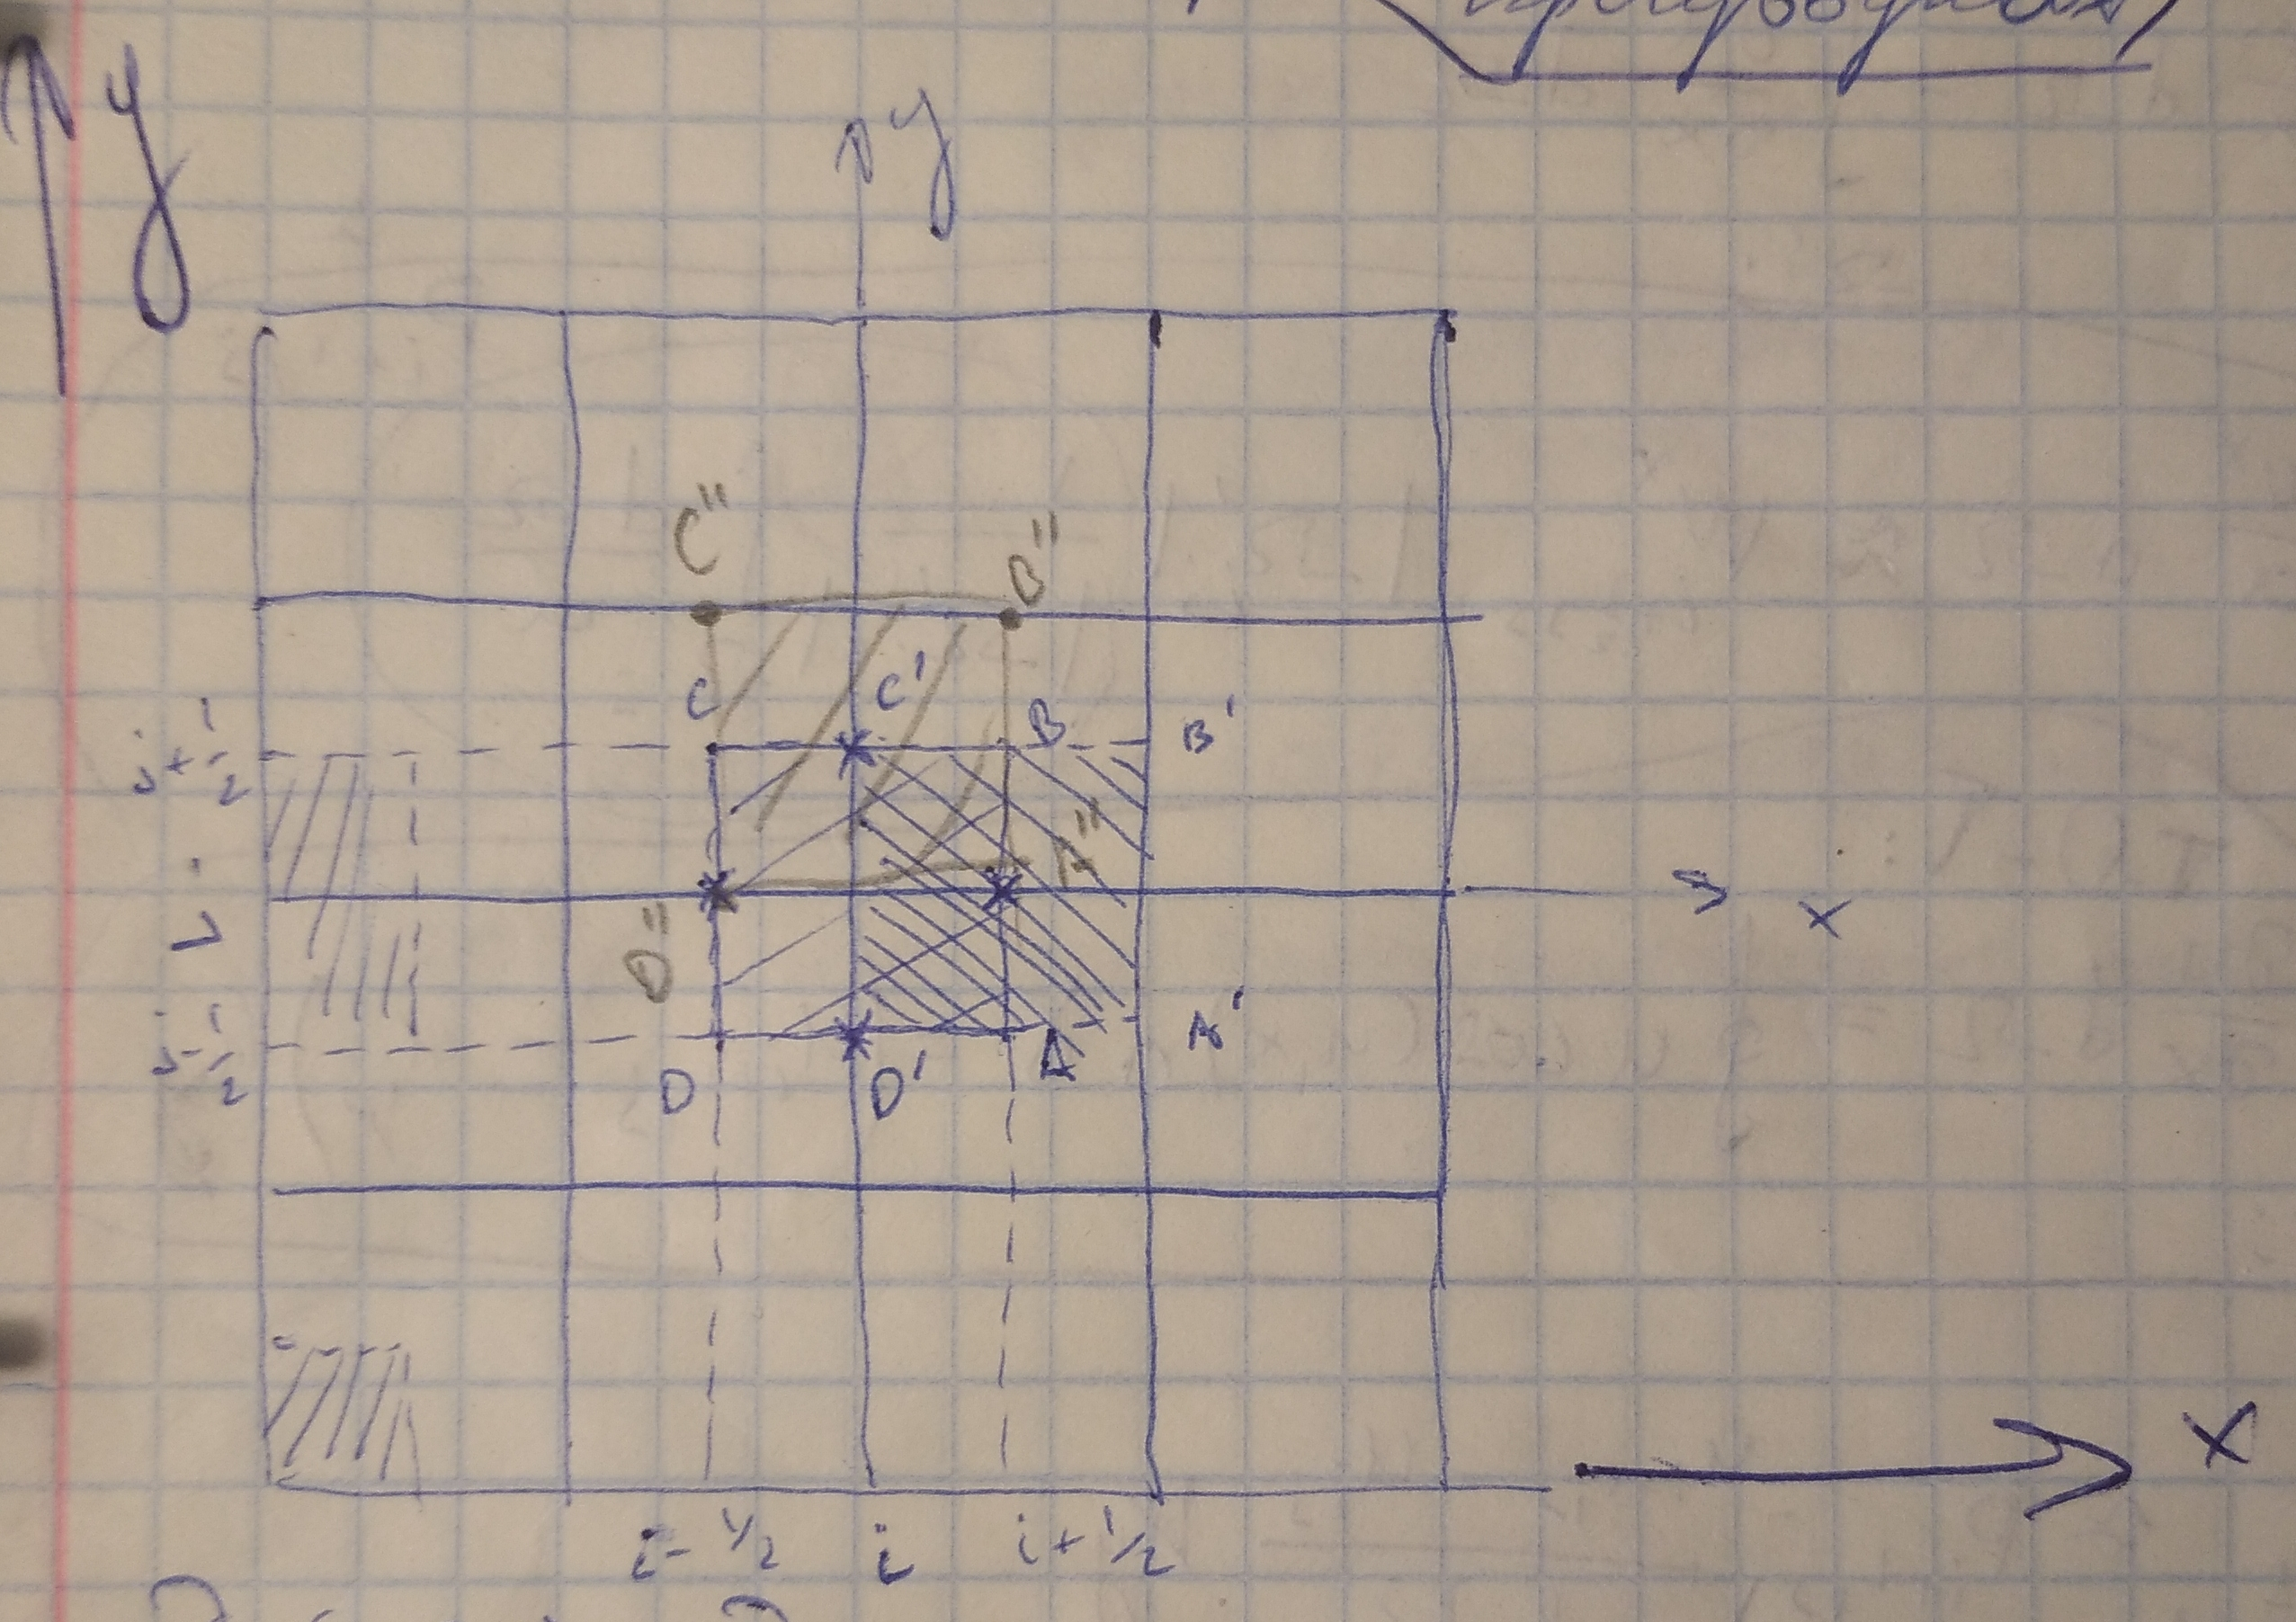
\includegraphics[scale = 0.2]{image.jpg}}
\caption{Илюстрация рассматриваемого конечного объёма}
\end{figure} 

Проинтегрируем уравнение 1 по конечному объёму и домножим на -1:
\begin{equation}
\int\limits_{\Omega_{ij}}{\left[ \dfrac{\partial}{\partial x}\left( a\dfrac{\partial u}{\partial x}\right) + \dfrac{\partial}{\partial y}\left( b\dfrac{\partial u}{\partial y}\right) \right]d\Omega}
 - \int\limits_{\Omega_{ij}}qud\Omega = \int\limits_{\Omega_{ij}}fd\Omega 
\end{equation}

Подробнее рассмотрим первое слагаемое из левой части. Под интегралом стоит дивергенция, применяем формулу Остроградского-Гаусса и получаем следующее выражение:
$\oint\limits_{\gamma_{ij}}{\left[ a\dfrac{\partial u}{\partial x}cos(n,x) + b\dfrac{\partial u}{\partial y}cos(n,y) \right]d\gamma}$.
Выполняем замену переменных: 
\begin{equation}\label{eq4}
\left[ \omega^x = a\dfrac{\partial u}{\partial x}; \omega^y =  b\dfrac{\partial u}{\partial y} \right]
\end{equation}
и приближённо вычисляем интегралы по границе (отдельно для каждого из двух слагаемых под интегралом). Заметим, что, с учётом граничных нормалей, в первом интеграле останется только два слагаемых(по левой и правой границам конечного объёма $\Omega_{i,j}$), как, впрочем, и во втором(но уже по верхней и нижней границам). Таким образом, приходим к следующей формуле.
 
\begin{equation}\label{eq3}
\oint\limits_{\gamma_{ij}}{\left[ a\dfrac{\partial u}{\partial x}cos(n,x) + b\dfrac{\partial u}{\partial y}cos(n,y) \right]d\gamma} 
 = \left( w_{i+0.5,j}^x - w_{i-0.5,j}^x \right) h_y + 
\left( w_{i,j+0.5}^y - w_{i,j-0.5}^y \right) h_x 
\end{equation}

Где, в частности, $w_{i+0.5,j}^x$ - значение $w^x$ в средней точке соответсвующего участка границы

С учётом замены (\ref{eq4}), легко видеть, что выполнены следующие равенства:

\begin{equation}\label{eq1}
\int\limits_{\Omega_{ij}^{'}}{\dfrac{\omega^x}{a}d\Omega} = \int\limits_{\Omega_{ij}^{'}}{\dfrac{\partial u}{\partial x}d\Omega} 
\end{equation}
\begin{equation}\label{eq2}
\int\limits_{\Omega_{ij}^{''}}{\dfrac{\omega^y}{b}d\Omega} = \int\limits_{\Omega_{ij}^{''}}{\dfrac{\partial u}{\partial y}d\Omega}
\end{equation}

В формулах (\ref{eq1}), (\ref{eq2}) - $\Omega_{ij}^{'}$ и $\Omega_{ij}^{''}$ это конечные объёмы, сдвинутые на половину шага в направлении оси Ох и Оy соответственно. Также, эти конечные объёмы изображениы на рисунке (\ref{fig1}).
Рассмотрим подробнее (\ref{eq1}). Применяя к правой части теорему О-Г., а левую часть преобразовав определённым образом, получаем уже конечно-разностное выражение.

$$
(\ref{eq1}) \Longleftrightarrow \omega_{i+0.5,j}^x \cdot \int\limits_{\Omega_{ij}^{'}}{\dfrac{d\Omega}{a}} = (v_{i+1,j} - v_{ij})h_y
$$

Отсюда легко можно найти выражение для $\omega_{i+0.5,j}^x$, посчитав численно интеграл. Точно также рассматриваем (\ref{eq2}). Обозначив 
$$
p_{i+0.5, j} = \dfrac{h_xh_y}{\int\limits_{\Omega_{ij}^{'}}{\dfrac{d\Omega}{a}}} ; \quad
q_{i, j+0.5} = \dfrac{h_xh_y}{\int\limits_{\Omega_{ij}^{''}}{\dfrac{d\Omega}{b}}}; 
$$ 
получаем уравнение(для $p_{i-0.5, j}$ и $q_{i, j-0.5}$ выражения аналогичны, изменятся только конечные объёмы, т.е. будут "сдвиги" в другом направлении):

\begin{eqnarray}
\dfrac{1}{h_x^2}(p_{i+0.5,j}(v_{i+1,j}-v_{i,j}) - p_{ij}(v_{i,j}-v_{i-1,j})) +
\dfrac{1}{h_y^2}(q_{i,j+0.5}(v_{i,j+1}-v_{i,j}) - q_{ij}(v_{i,j}-v_{i,j-1})) + \nonumber
\\
+ \dfrac{\rho_{ij}}{h_xh_y}v_{ij}= \dfrac{g_{ij}}{h_xh_y}
\end{eqnarray}

Сгруппировав слагаемые при соответствующих узновых точках, получим:

\begin{eqnarray}
 - \left( \dfrac{p_{i-0.5, j}v_{i-1,j} + p_{i+0.5, j}v_{i+1,j}}{h_x^2} + \dfrac{q_{i, j+0.5}v_{i,j+1} + q_{i, j-0.5}v_{i,j-1}}{h_y^2} \right) + \nonumber 
\\
+ \left( \dfrac{p_{i+0.5, j} + p_{i-0.5, j}}{h_x^2} + \dfrac{q_{i, j+0.5} + q_{i, j-0.5}}{h_y^2} + \dfrac{\rho_{ij}}{h_xh_y} \right) v_{ij}
 = \dfrac{g_{ij}}{h_xh_y}
\end{eqnarray}

Все вышеперечисленные выражения я привёл в общем виде для упрощения восприятия. Теперь рассмотрим, чему равны коэффициенты в контексте конкретной задачи.

\begin{equation}
\begin{cases}
p_{i+0.5,j} = \int\limits_{\Omega_{ij}^{'}}{\dfrac{d\Omega}{x + y}} &
p_{i-0.5,j} = \int\limits_{\Omega_{i-1,j}^{'}}{\dfrac{d\Omega}{x + y}} \\
q_{i,j+0.5} = \int\limits_{\Omega_{ij}^{''}}{\dfrac{d\Omega}{1 + xy}} &
q_{i,j-0.5} = \int\limits_{\Omega_{i,j-1}^{''}}{\dfrac{d\Omega}{1 + xy}} \\
\rho_{ij} = \int\limits_{\Omega_{ij}}{x^4 d \Omega} \\
g_{ij} = \int\limits_{\Omega_{ij}}{fd \Omega} 
\end{cases}
\end{equation}

Замечание о численном вычислении интегралов. Я вычисляю интегралы по следующей формуле (Формула Гаусса для двумерного случая):

\begin{equation}
\int\limits_{[x_0; x_1] \times [y_0; y_1]}{\phi(x, y)d\Omega} = \dfrac{(x_1-x_0)(y_1-y_0)}{4} \sum\limits_{i=1}^4\phi\left(x_0 + \dfrac{(\xi_i+1)(x_1-x_0)}{2} ,y0 + \dfrac{(\eta_i+1)(y_1-y_0)}{2} \right)
\end{equation}
Где $\xi_i$ и $\eta_i$ представляют все пары вида $\left(\dfrac{\pm 1}{\sqrt{3}}; \dfrac{\pm 1}{\sqrt{3}}\right)$

Тут используется отображение иходного прямоугольника на базисный. Для этого используются следующие формулы:

\begin{equation}
\begin{cases}
\xi(x, y) = 2 \dfrac{x - x_0}{x_1-x_0} - 1 \\
\eta(x, y) = 2 \dfrac{y - y_0}{y_1-y_0} - 1
\end{cases}
\end{equation}

Подробнее про то, как получить эту формулу можно посмотреть, например, тут :
\url{https://ru.wikipedia.org/wiki/%D0%A1%D0%BF%D0%B8%D1%81%D0%BE%D0%BA_%D0%BA%D0%B2%D0%B0%D0%B4%D1%80%D0%B0%D1%82%D1%83%D1%80%D0%BD%D1%8B%D1%85_%D1%84%D0%BE%D1%80%D0%BC%D1%83%D0%BB}

\section{Метод Якоби}

Приведём общую схему метода Якоби в матричном виде. В методе Якоби в качестве предобуславлевателя берём диагональную матрицу $D$:

\begin{equation}
v^{k+1} = D^{-1}(g - (L+U)v^k)
\end{equation}

Ниже привожу несколько иллюстраций для пояснений.

\begin{figure}[H]
\begin{minipage}[H]{0.59\linewidth}
\center{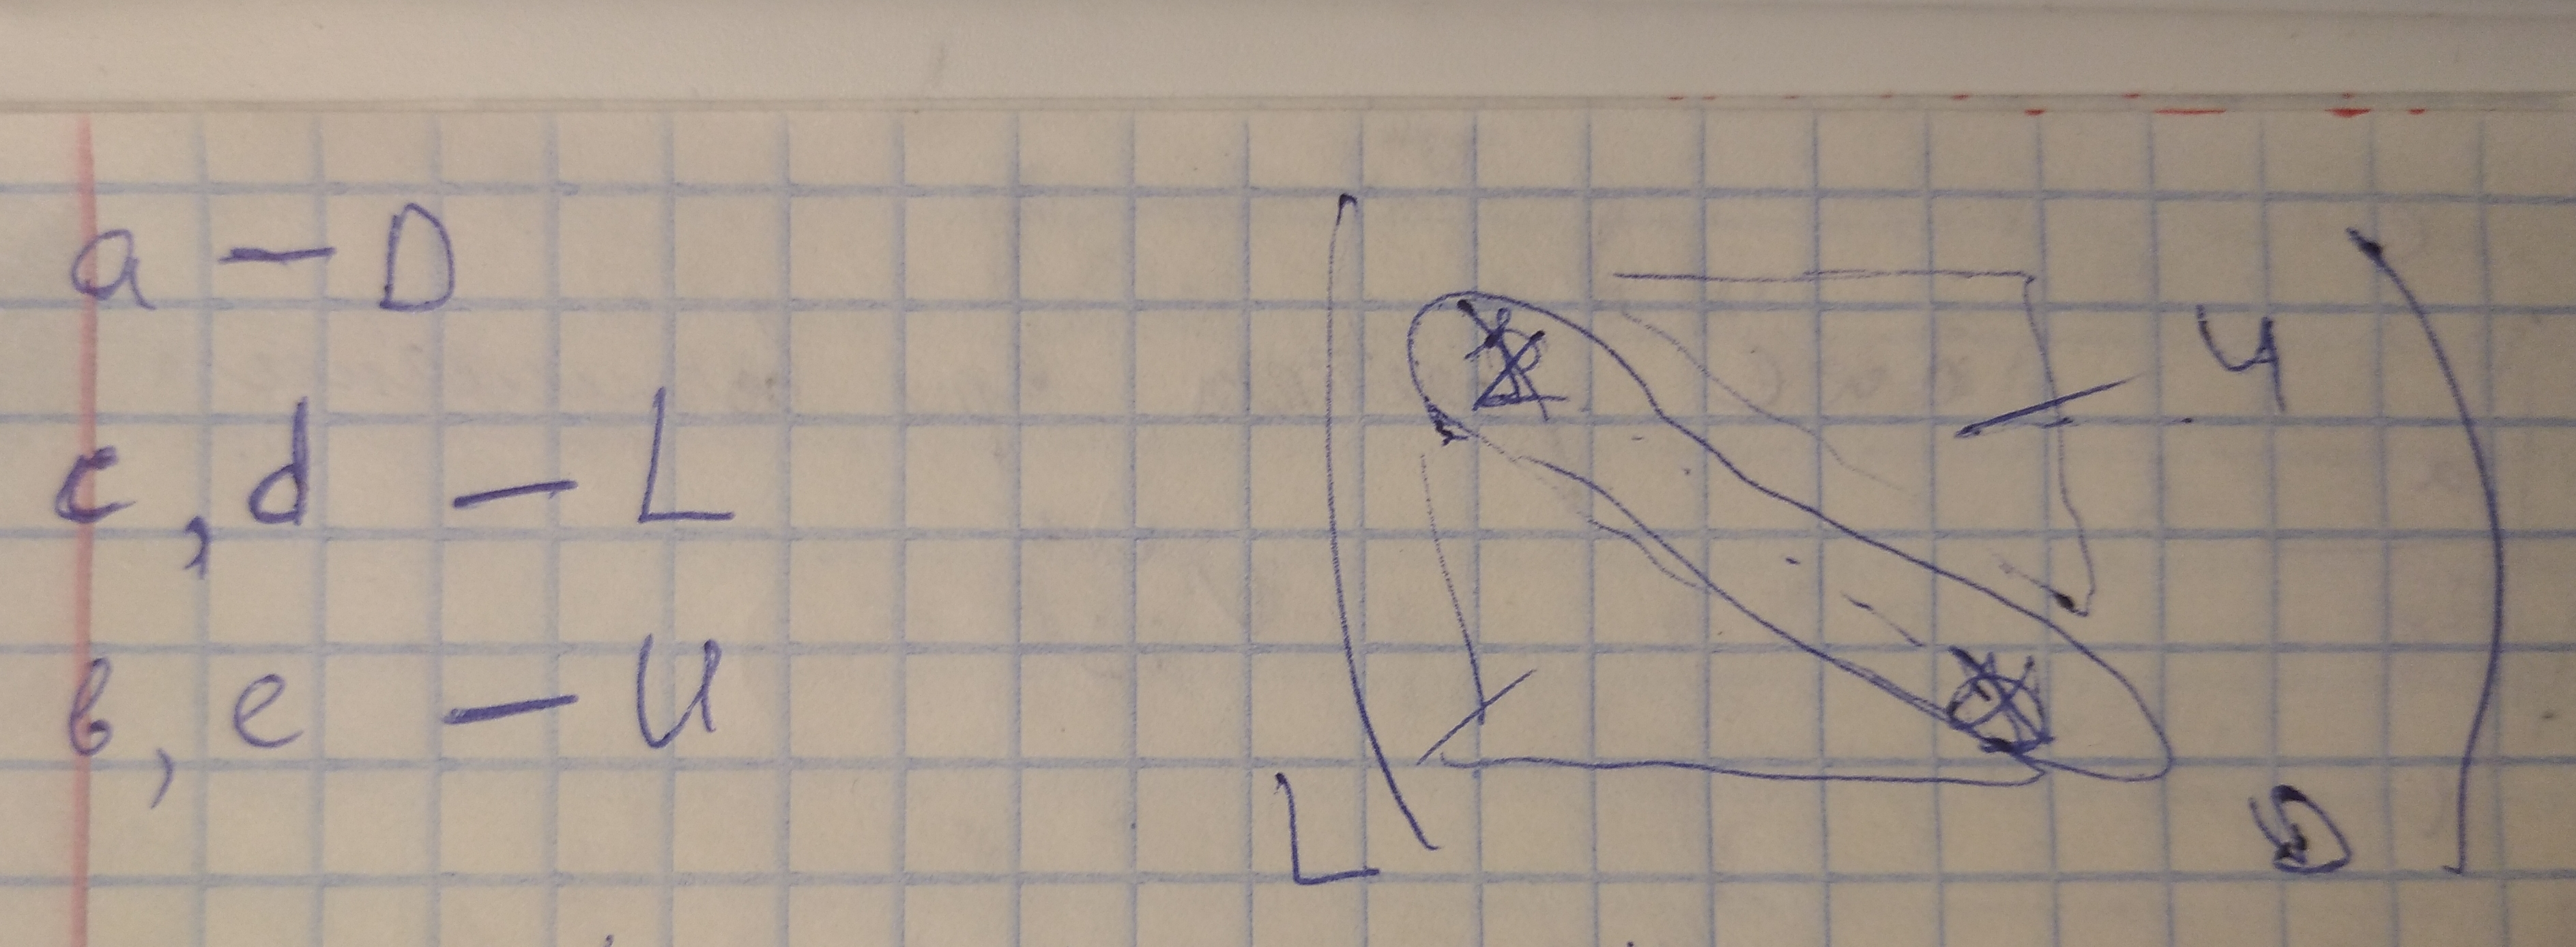
\includegraphics[width=0.8\linewidth]{image2.jpg} \\ a) Матричный вид коэффициентов}
\end{minipage}
\hfill
\begin{minipage}[H]{0.39\linewidth}
\center{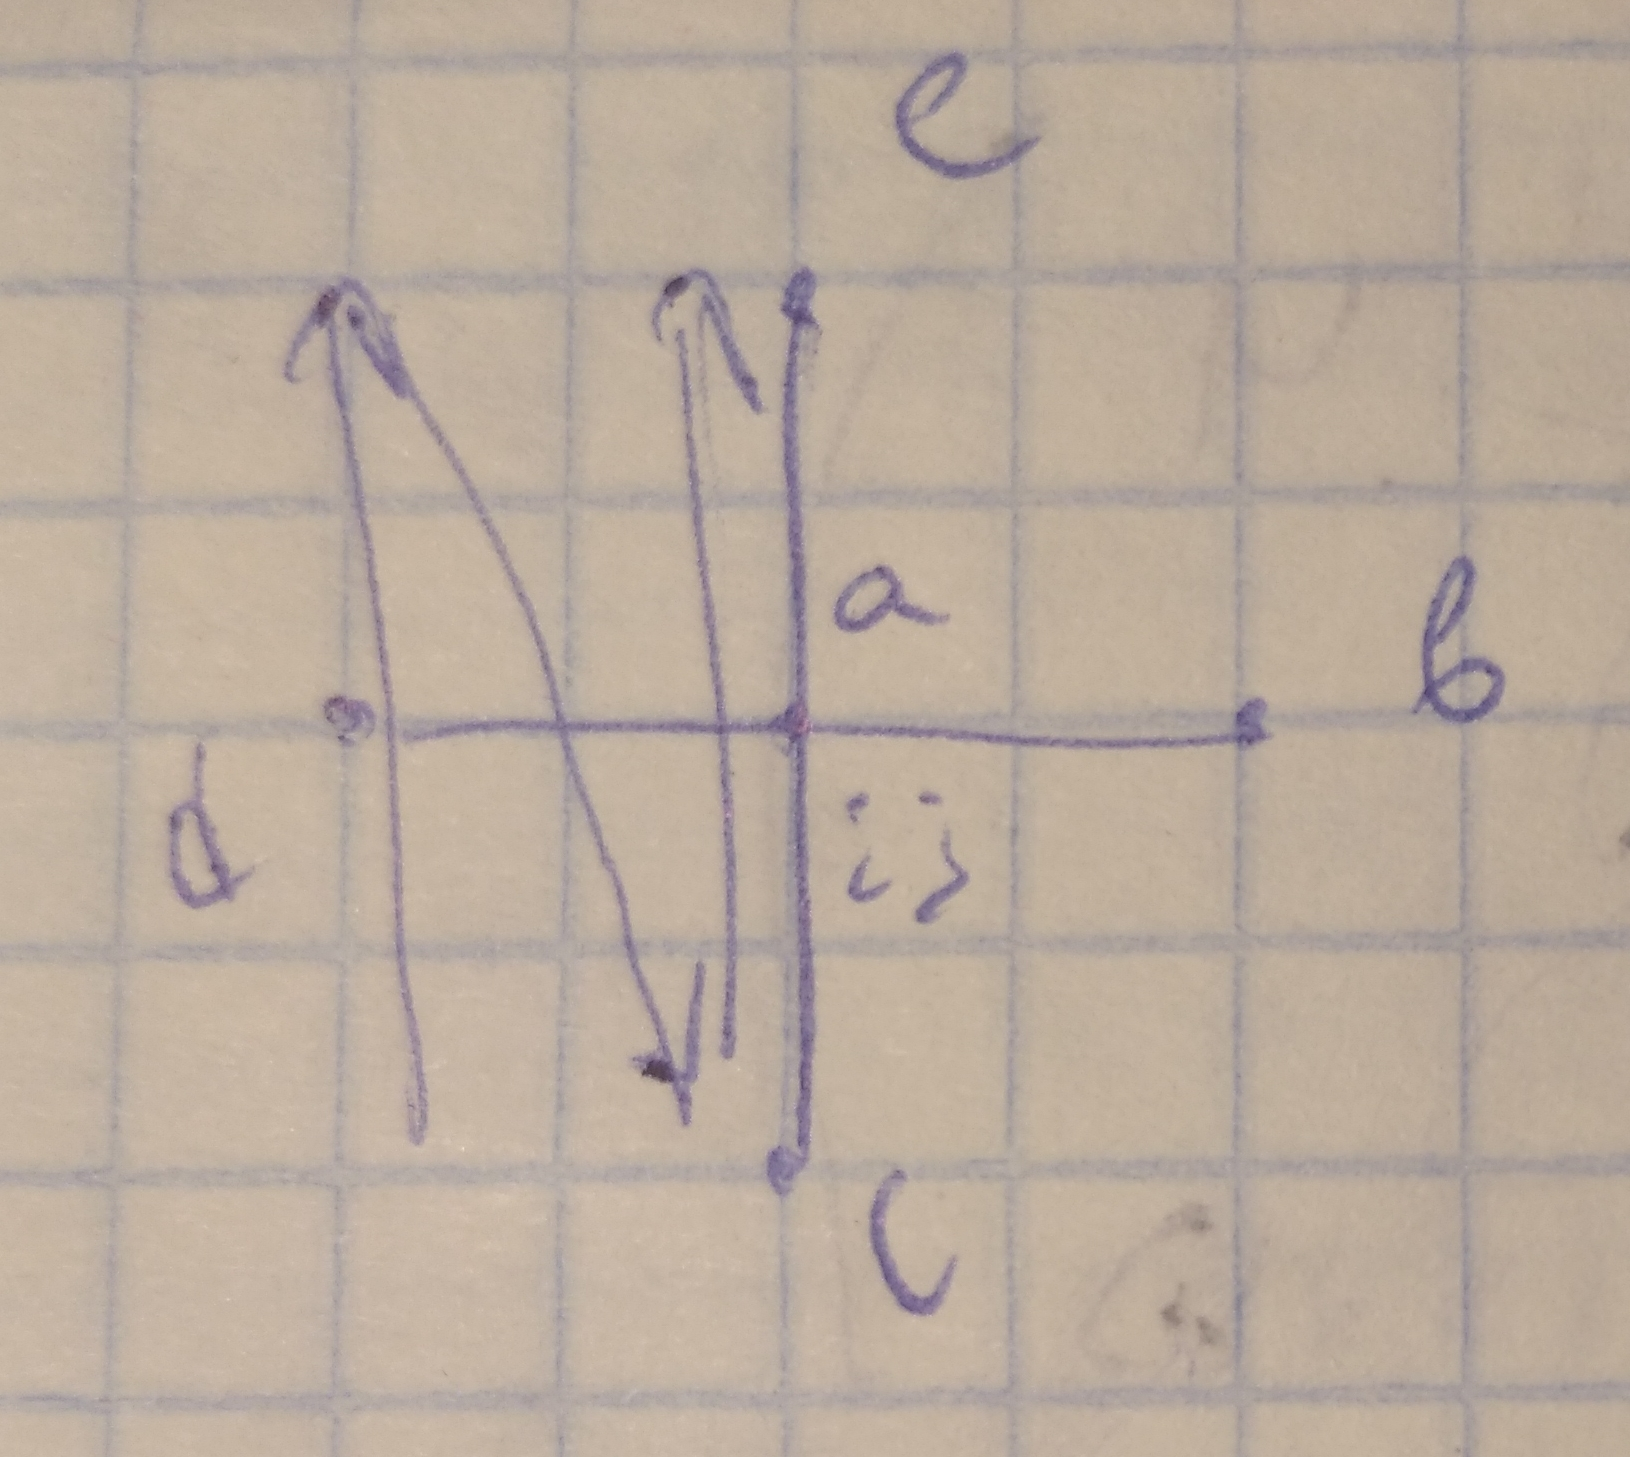
\includegraphics[width=0.5\linewidth]{image3.jpg} \\ b) Порядок обхода}
\end{minipage}
\end{figure} 


Будем применять итерационную процедуру метода Якоби в следующем виде.

\begin{equation}
v_{i,j}^{k+1} = \dfrac{1}{A_{i,j}} \cdot (G_{i,j} - D_{i,j}v_{i-1,j}^{k} - C_{i,j}v_{i,j-1}^{k} - E_{i,j}v_{i,j+1}^{k} - B_{i,j}v_{i+1,j}^{k})
\end{equation}

\section{Метод Зейделя}

Будем применять итерационную процедуру метода Зейделя в следующем виде:

\begin{equation}
v_{i,j}^{k+1} = \dfrac{1}{A_{i,j}} \cdot (G_{i,j} - D_{i,j}v_{i-1,j}^{k+1} - C_{i,j}v_{i,j-1}^{k+1} - E_{i,j}v_{i,j+1}^{k} - B_{i,j}v_{i+1,j}^{k})
\end{equation}

Заметим, что соответствующие значения $v$ при коэффициентах $C$ и $D$ на момент расчёта $v_{i,j}$ уже известны.

\section{Метод SOR}

В случае метода Зейделя, предобуславиливатель имеет вид: $B := L + D$. В матричном виде выражение для $k+1$ го приближения записывается так:

\begin{equation}
v^{k+1} = D^{-1}(g - Uv^k - Lv^{k+1})
\end{equation}

Будем применять итерационную процедуру метода SOR в следующем виде:

\begin{eqnarray}
\begin{cases}
v_{Z, i, j}^{k+1} = \dfrac{1}{A_{i,j}} \cdot (G_{i,j} - D_{i,j}v_{Z,i-1,j}^{k+1} - C_{i,j}v_{Z, i,j-1}^{k+1} - E_{i,j}v_{SOR,i,j+1}^{k} - B_{i,j}v_{SOR,i+1,j}^{k}) \\
v_{SOR}^{k+1} = v_{SOR}^{k} + \omega (v_{Z}^{k+1} - v_{SOR}^{k}) 
\end{cases}
\end{eqnarray}

Где $v_{Z}$ - вычисляется по методу Зейделя

\section{Результаты}
\subsection{Метод Якоби}

Для достижения точности $\varepsilon = 10^{-3}$ возьмём чило разбиений равным $N = 100$ и $\varepsilon_{iter} = \dfrac{10^{-4}\pi^2}{2N^2}$. 

\begin{figure}[H]
\centerline{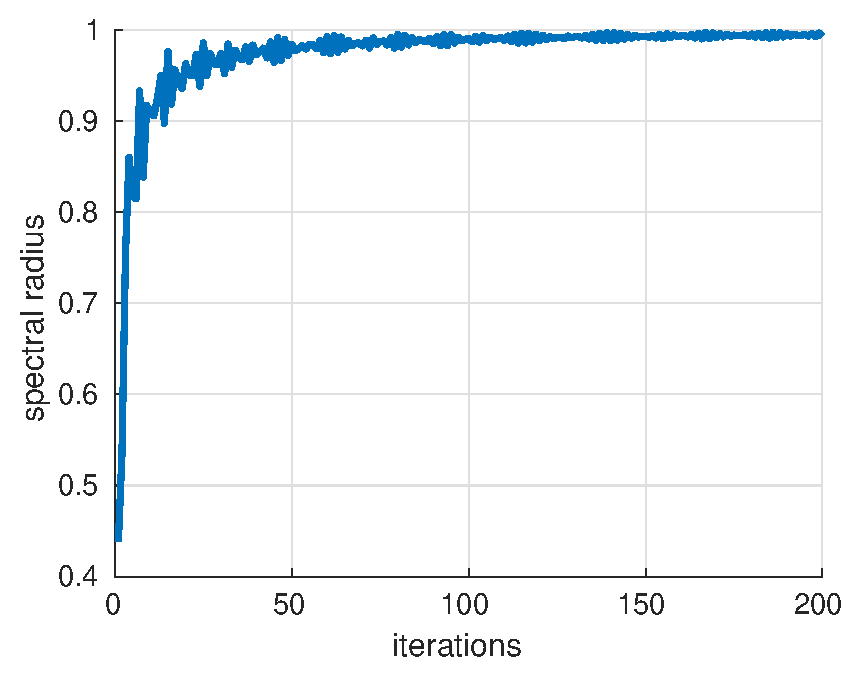
\includegraphics[scale = 0.8]{jacobiSpectre.eps}}
\caption{Зависимость спектрального радиуса от числа итераций}
\label{fig4}
\end{figure} 

При этом $\rho_{J} = \lim\limits_{k\rightarrow \inf}{\dfrac{||v^{k+1} - v^{k}||}{||v^{k} - v^{k-1}||}} = 0.99945 \approx 0.99950 $, что согласуется с теоретическим значением.
 
\subsection{Метод Зейделя}

Для достижения точности $\varepsilon = 10^{-3}$ возьмём чило разбиений равным $N = 100$ и $\varepsilon_{iter} = \dfrac{10^{-4}\pi^2}{N^2}$. 

\begin{figure}[H]
\centerline{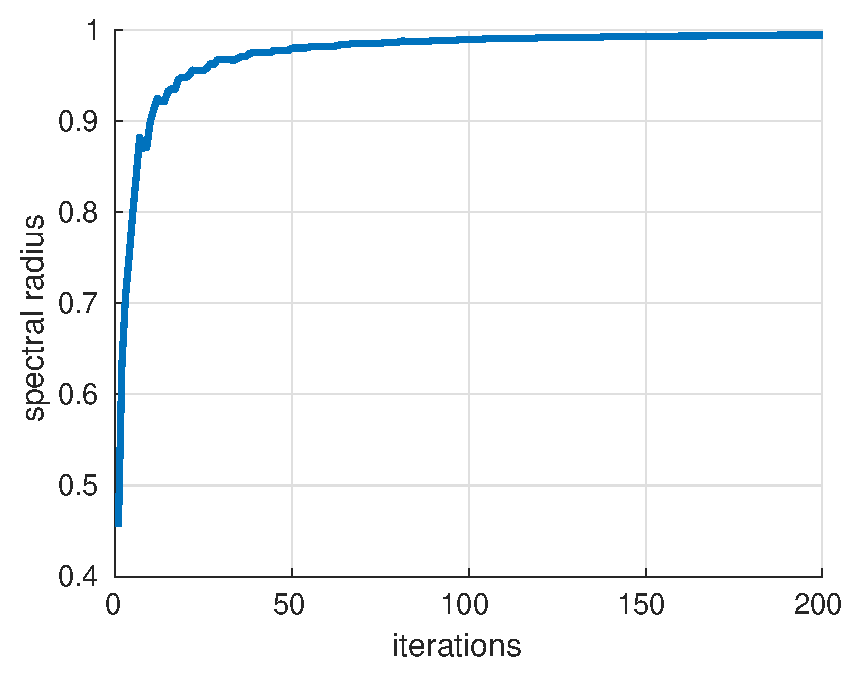
\includegraphics[scale = 0.8]{zeidelSpectre.eps}}
\caption{Зависимость спектрального радиуса от числа итераций}
\end{figure} 

При этом $\rho_{Z} = \lim\limits_{k\rightarrow \inf}{\dfrac{||v^{k+1} - v^{k}||}{||v^{k} - v^{k-1}||}} = 0.99855 \approx 0.9990 = \rho_{J}^2$, что согласуется с теоретическим значением.

\subsection{Метод SOR}

Для достижения точности $\varepsilon = 10^{-3}$ возьмём чило разбиений равным $N = 100$ и $\varepsilon_{iter} = \dfrac{10^{-7}\pi}{N}$.

\textbf{Примечание к рисунку (\ref{fig5}):}

В ходе исследований метода SOR, я пытался получить графическую оценку параметра релаксации, максимально близкую к теоретическому значению. Если строить график, используя число разбиений из предыдущих пунктов (а именно $N = 100$), то я получал значение $\omega_{opt} \approx 1.5$. Тогда я решил немного поэкспериментировать со значениями числа разбиений, И при $N = 28$ мне удалось достичь приведённых ниже значений. Тоесть, рисунок (\ref{fig5}) построен для $N = 28$. И тогда получается, что методу Зейделя для такого числа разбиений потребуется $\approx 1000$ итераций для достижения условия выхода из итерационного процесса. 

А в таблице (\ref{tb1}) я привожу число итераций для всех методов при $N = 100$, так что никаких противоречий в итоге не возникает.



\begin{figure}[H]
\centerline{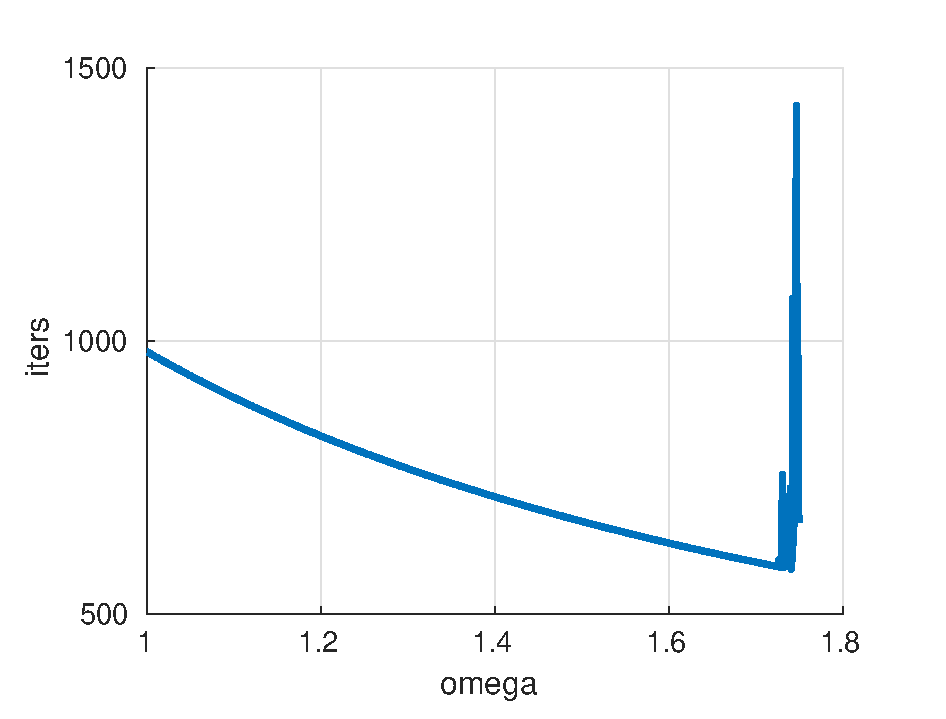
\includegraphics[scale = 0.8]{sor.eps}}
\caption{Зависимость числа итераций $n(\varepsilon)$ от параметра релаксации $\omega$}
\label{fig5}
\end{figure} 

\begin{figure}[H]
\centerline{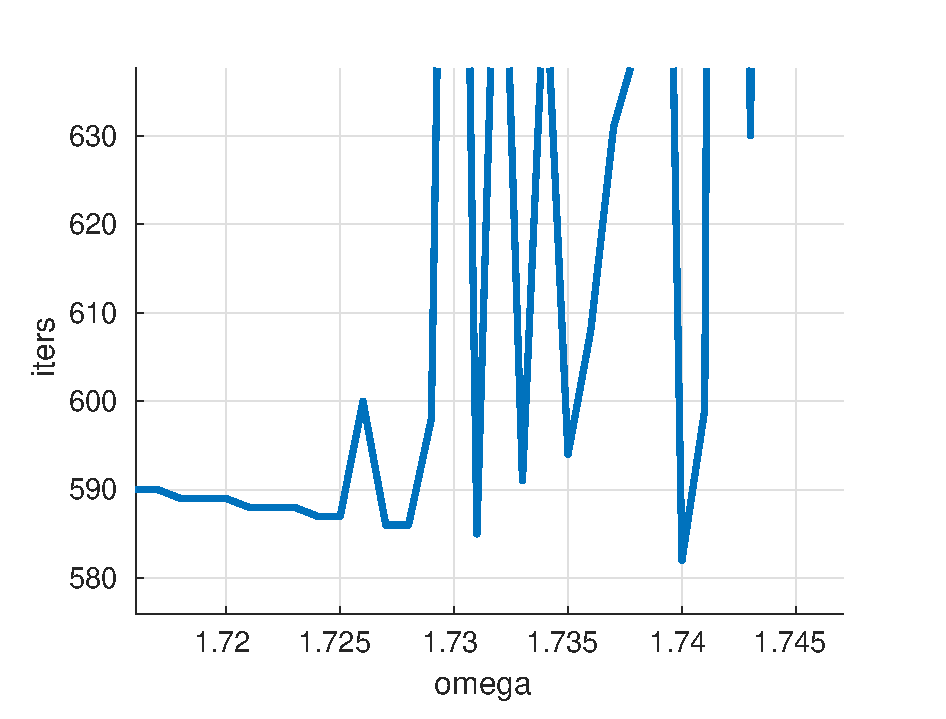
\includegraphics[scale = 0.8]{sor2.eps}}
\caption{Зависимость числа итераций $n(\varepsilon)$ от параметра релаксации $\omega$ (приближение)}
\label{fig2}
\end{figure} 

\begin{figure}[H]
\centerline{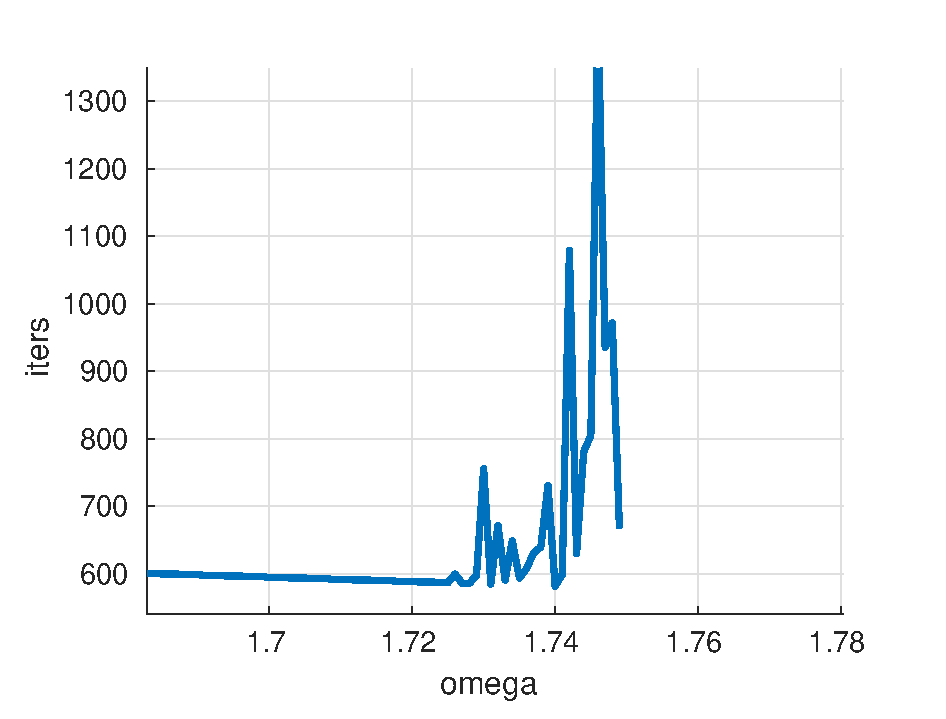
\includegraphics[scale = 0.8]{sor3.eps}}
\caption{Зависимость числа итераций $n(\varepsilon)$ от параметра релаксации $\omega$ (приближение 2)}
\label{fig3}
\end{figure} 

По графику (\ref{fig2}) видно, что оптимальным параметром релаксации будет $\omega = 1.725$. Однако, из теории следует, что оптимальный параметр должен равняться: $\omega_{opt} = \dfrac{2}{1+\sqrt{1 - \rho_{Z}}} \approx 1.9387$. Я пытался добиться большей точности от графического метода нахождения $\omega_{opt}$ изменяя $N$ и $\varepsilon_{iter}$, но мои попытки не принесли результатов, так как схема начинала терять устойчивость. Я думаю, что всё дело в выбранной мной конкретной задаче, и можно было бы теоретически подобрать исходную задачу точнее, чтобы получить лучший результат. Я же буду далее использовать полученное мною значение $\omega_{opt} = 1.725$.

Также привожу рисунок (\ref{fig3}) для иллюстрации неустойчивости. Я уменьшил шаг дискретизаци до $\dfrac{1}{1000}$, и при таком шаге уже можно заметить определённые моменты. Видно, что с каждым шагом точки графика совершают колебания с растущей амплитудой. Тоесть, имеем не излом, а некоторые колебания графика, если бы их не было, график начал бы монотонно возрастать. Подобное поведение также наблюдается на рисунке (\ref{fig4})
\subsection{Сравнение методов}

\begin{table}[H]
\caption{Сравнение методов}
\begin{center}
\begin{tabular}{|c|c|c|c|}
\hline
Метод & $\rho$ & $\varepsilon_{iter}$ & $n(\varepsilon)$ \\
\hline
Jacobi & 0.99945 & 4.934802e-08 & 17712 \\
\hline
Zeidel & 0.99855 & 9.869604e-08 & 8858 \\
\hline
SOR & 0.9744 & 1.121997e-08 & 445 \\
\hline
\end{tabular}
\end{center}
\label{tb1}
\end{table}


\begin{figure}[H]
\centerline{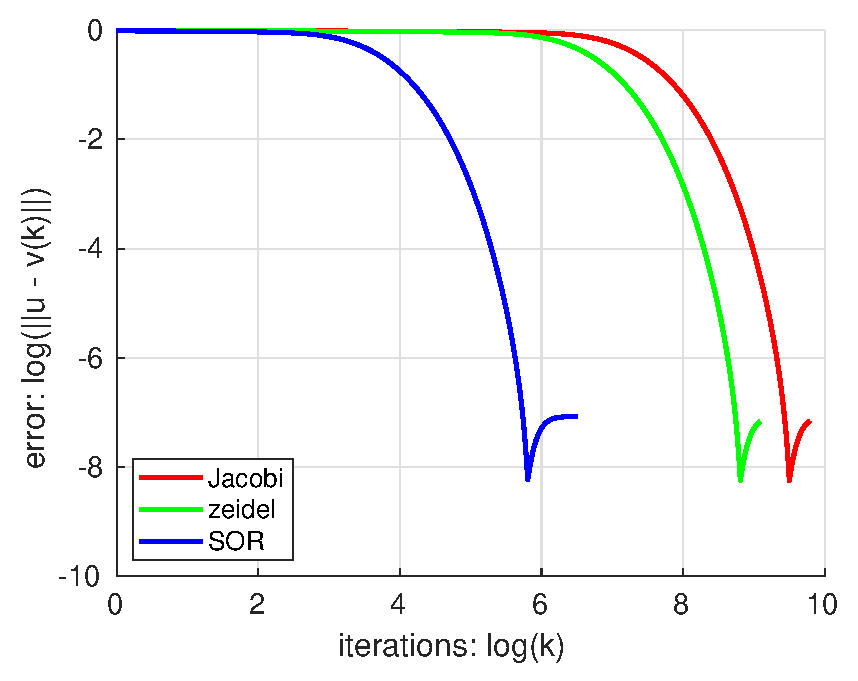
\includegraphics[scale = 0.8]{compare.eps}}
\caption{Сравнение зависимостей $||z^k||$ от числа итераций}
\end{figure}

\newpage

\section{Выводы}

В результате работы были рассмотрены 3 итерационных метода(Якоби, Зейделя, SOR) решения СЛАУ, построенной по МКО. Я получил полное соответствие практичеких и теоретических оценок скоростей сходимости методов, спектральных радиусов и соотношения числа итераций, за исключением $\omega_{opt}$. Как уже выше упоминалось, я считаю что это связано с конкретной задачей.

\section{Приложения}
Исходные файлы лабораторной работы можно найти тут: \\
\url{https://github.com/LanskovNV/numerical/tree/master/net_methods/lab_3}
\end{document}

